\section{Results}
\label{sec:results}

Table~\ref{tab:synth} contains the runtime, speedup, and efficiency of runs
produced by our parallel gspan algorithm on a synthetic dataset with
a support of 0.05.

\begin{table}
\centering
\begin{tabular}{cccc}
\hline
Cores & Runtime (seconds) & Speedup &  Eff.  \\
\hline
1    &   76.95   &  1.000 &     1.000  \\
2    &   51.89   &  1.483 &     0.741  \\
4    &   39.46   &  1.950 &     0.488  \\
8    &   31.36   &  2.454 &     0.307  \\
16   &   26.77   &  2.874 &     0.180  \\
32   &   24.15   &  3.186 &     0.100  \\
\hline
\end{tabular}
\caption{Runtime, speedup, and efficiency for synthetic dataset with support
         0.05.}
\label{tab:synth}
\end{table}

\begin{figure}
\centering
\begin{tabular}{ccc}
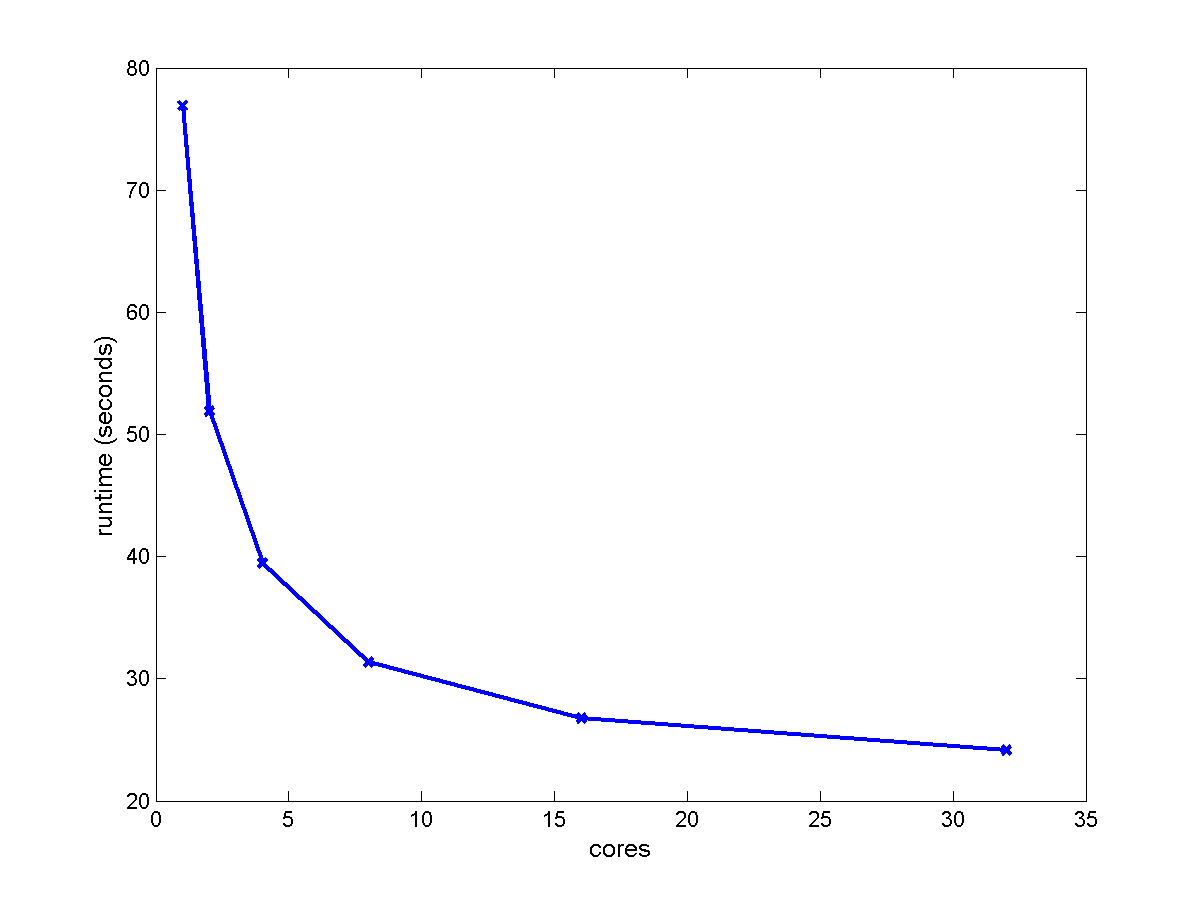
\includegraphics[width=0.3\textwidth]{synth_time.png} &
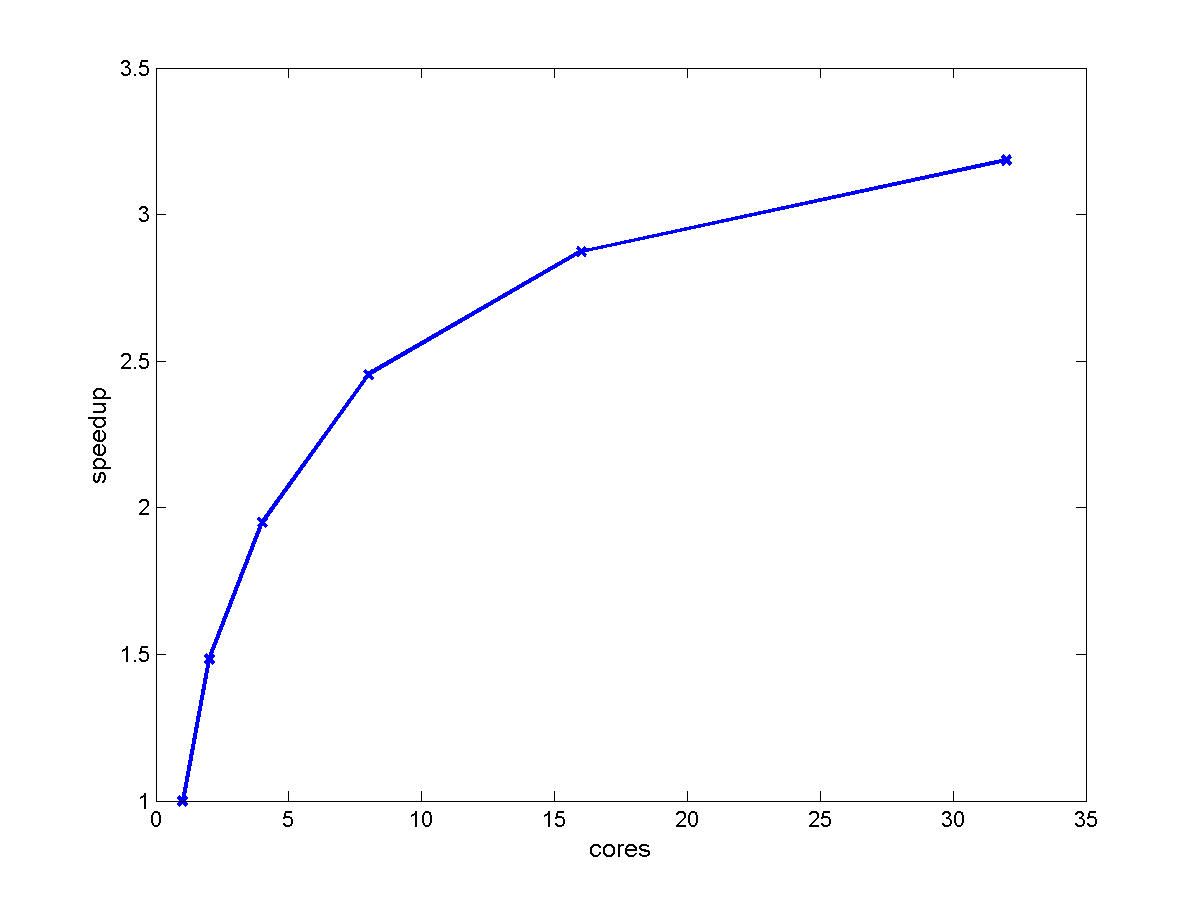
\includegraphics[width=0.3\textwidth]{synth_speedup.png} &
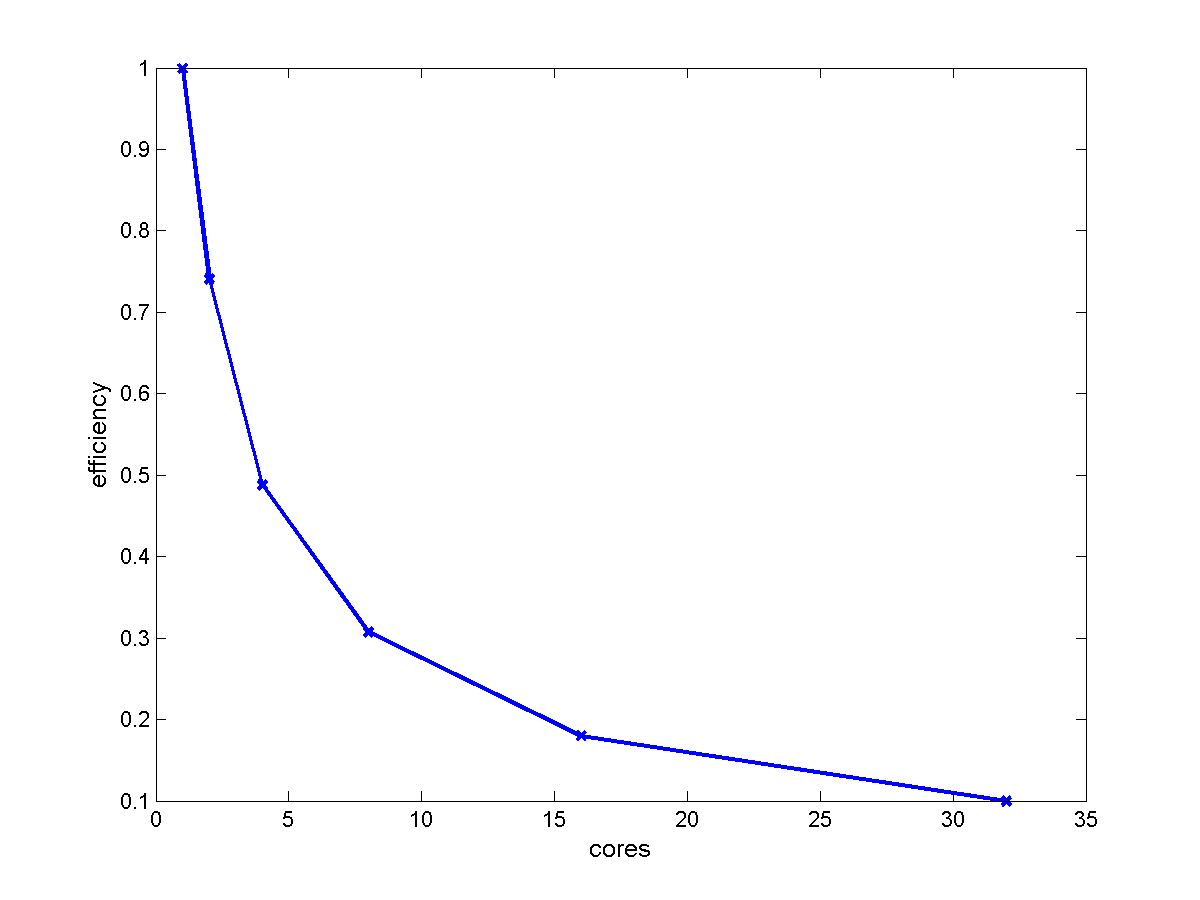
\includegraphics[width=0.3\textwidth]{synth_efficiency.png} \\
(a) & (b) & (c) \\
\end{tabular}
\caption{Plots of (a) runtime, (b) speedup, and (c) efficiency for
         synthetic dataset with support 0.05.}
\label{fig:synth}
\end{figure}

\begin{table}
\centering
\begin{tabular}{cccc}
\hline
Cores & Runtime (seconds) & Speedup &  Eff.  \\
\hline
 1    &   75.92    &  1.000 & 1.000 \\
 2    &   56.34    &  1.348 & 0.674 \\
 4    &   37.53    &  2.023 & 0.506 \\
 8    &   40.97    &  1.853 & 0.232 \\
16    &   31.16    &  2.436 & 0.152 \\
32    &   32.08    &  2.367 & 0.074 \\
\hline
\end{tabular}
\caption{Runtime, speedup, and efficiency for Compound\_422 dataset with support
         0.1.}
\label{tab:compound}
\end{table}

\begin{figure}
\centering
\begin{tabular}{ccc}
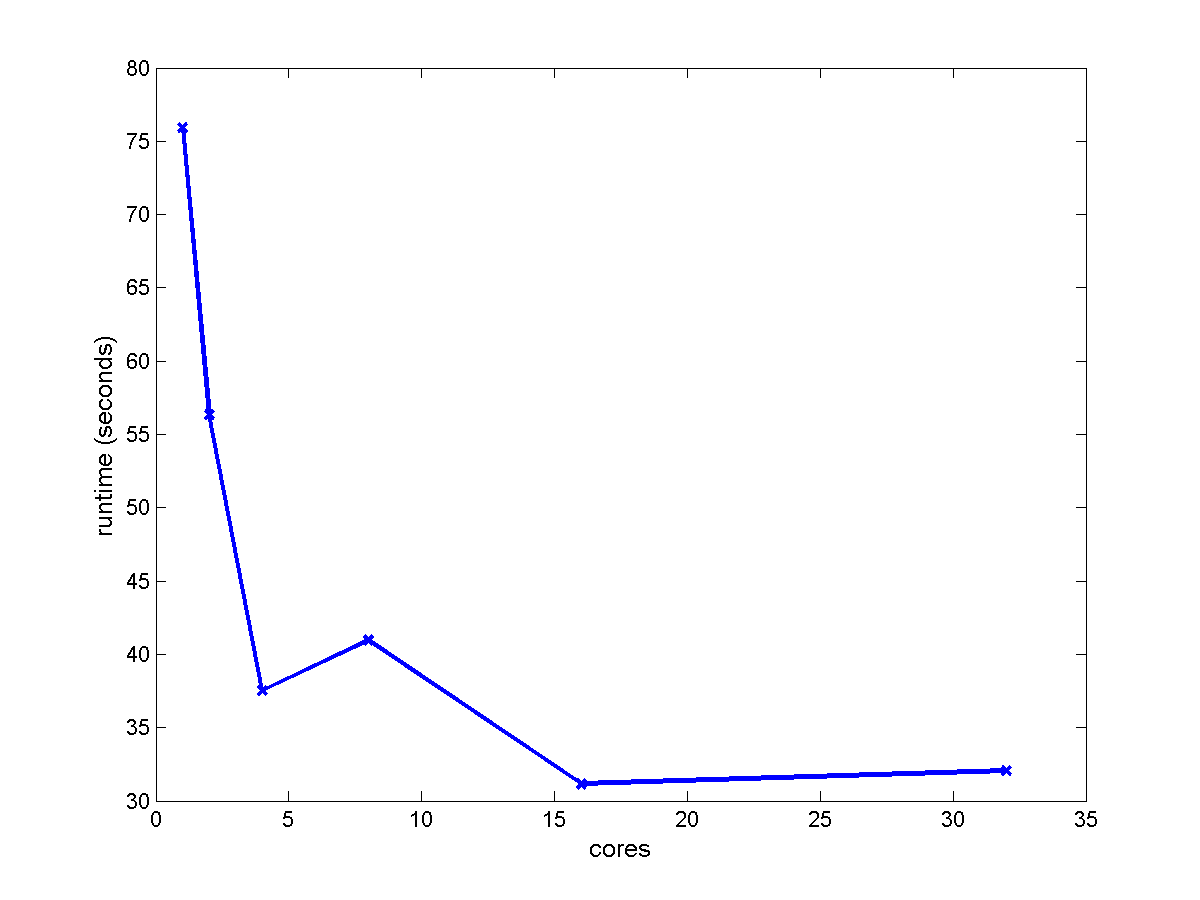
\includegraphics[width=0.3\textwidth]{compound_time.png} &
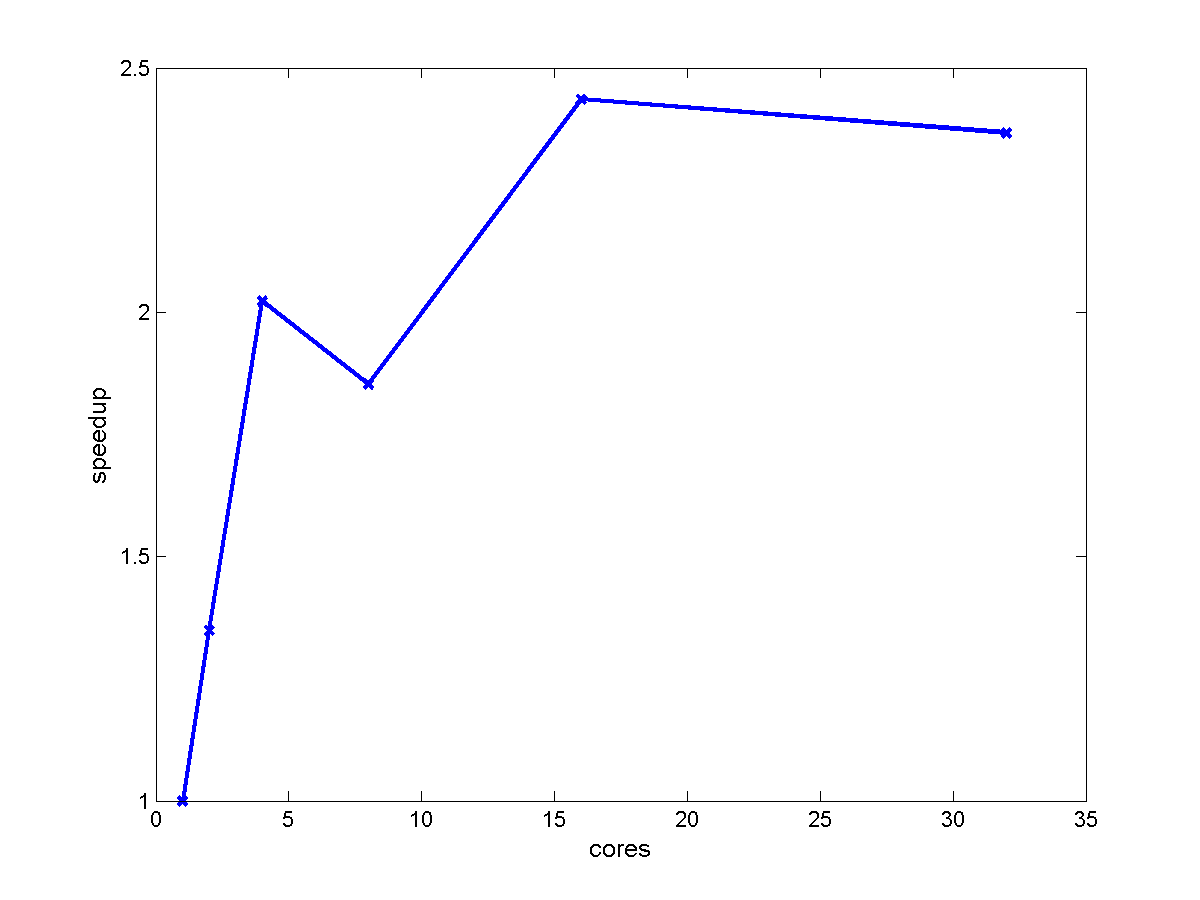
\includegraphics[width=0.3\textwidth]{compound_speedup.png} &
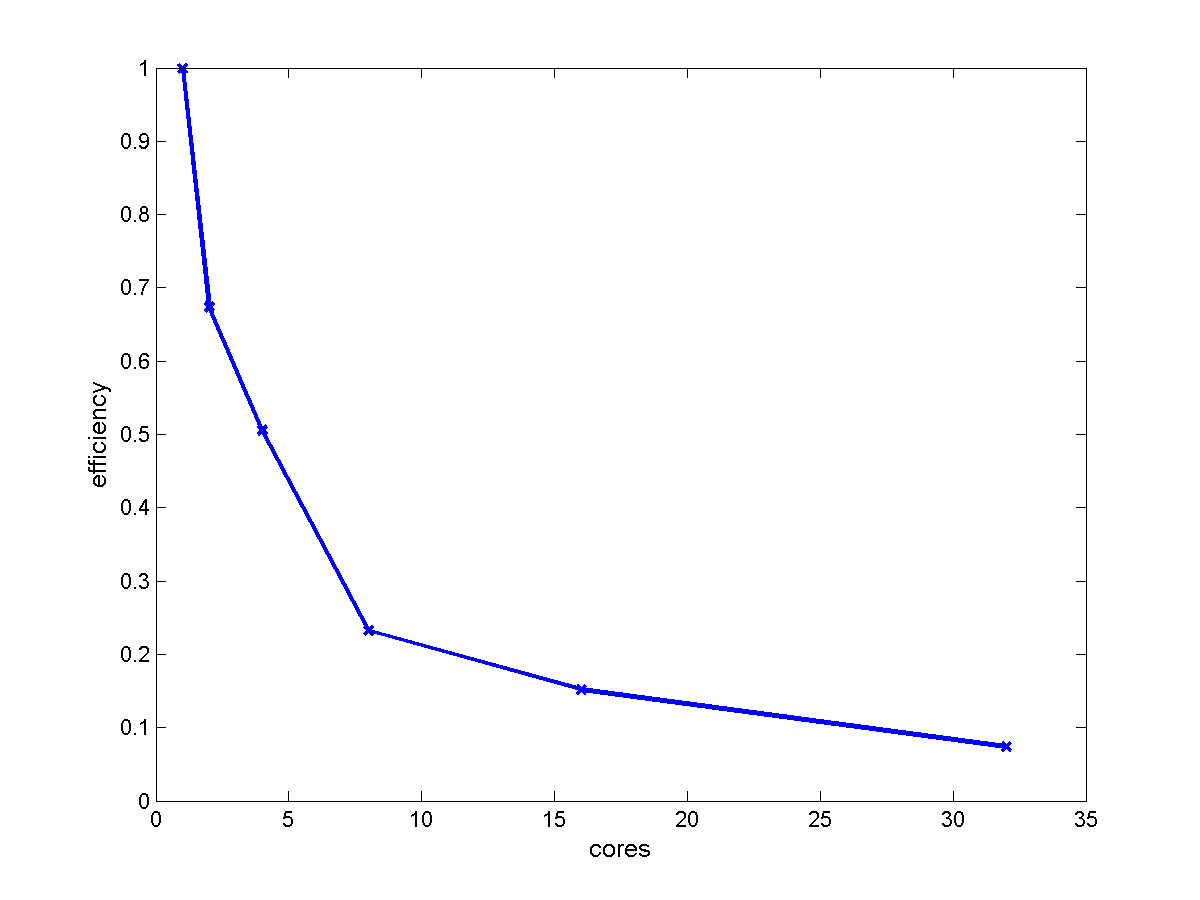
\includegraphics[width=0.3\textwidth]{compound_efficiency.png} \\
(a) & (b) & (c) \\
\end{tabular}
\caption{Plots of (a) runtime, (b) speedup, and (c) efficiency for
         Compound\_422 with support 0.1.}
\label{fig:compound}
\end{figure}


\begin{table}
\centering
\begin{tabular}{cccc}
\hline
Cores & Runtime (seconds) & Speedup &  Eff.  \\
\hline
 1    & 2503.03 & 1.000  & 1.000 \\
 2    & 2272.73 & 1.101  & 0.551 \\
 4    & 2239.04 & 1.118  & 0.279 \\
 8    & 2061.45 & 1.214  & 0.152 \\
16    & 2234.83 & 1.120  & 0.070 \\
32    & 2234.83 & 1.142  & 0.036 \\
\hline
\end{tabular}
\caption{Runtime, speedup, and efficiency for MCG-7 with support
         0.1.}
\label{tab:mcg7}
\end{table}

\begin{figure}
\centering
\begin{tabular}{ccc}
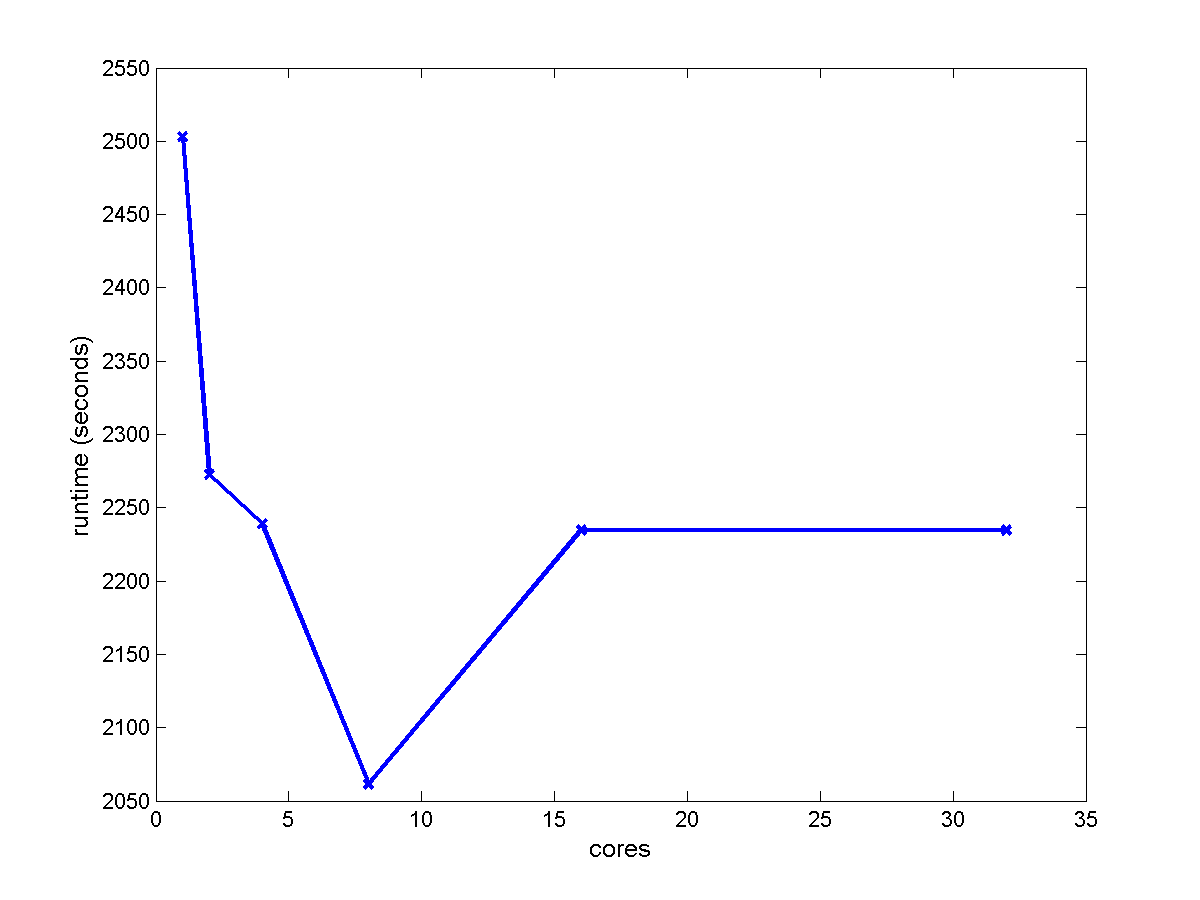
\includegraphics[width=0.3\textwidth]{mcg7_time.png} &
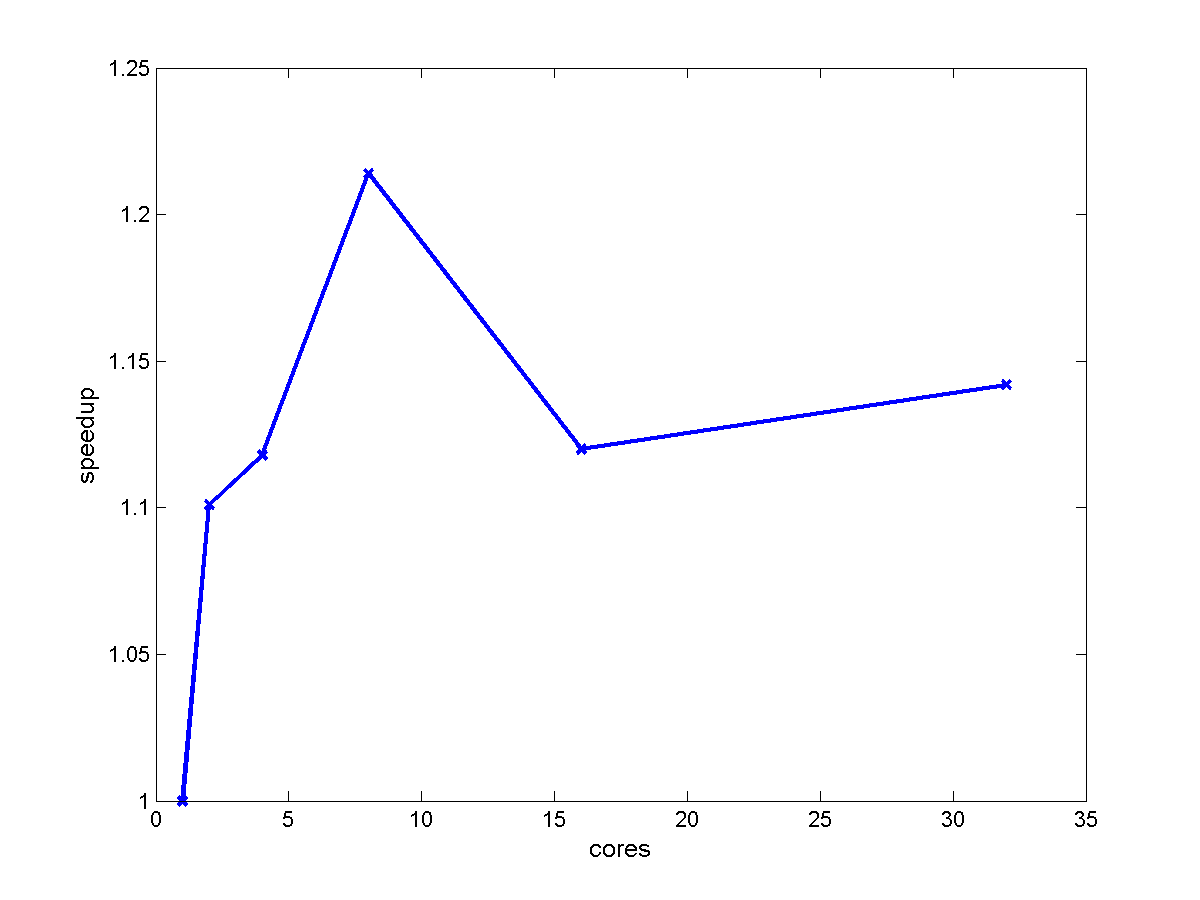
\includegraphics[width=0.3\textwidth]{mcg7_speedup.png} &
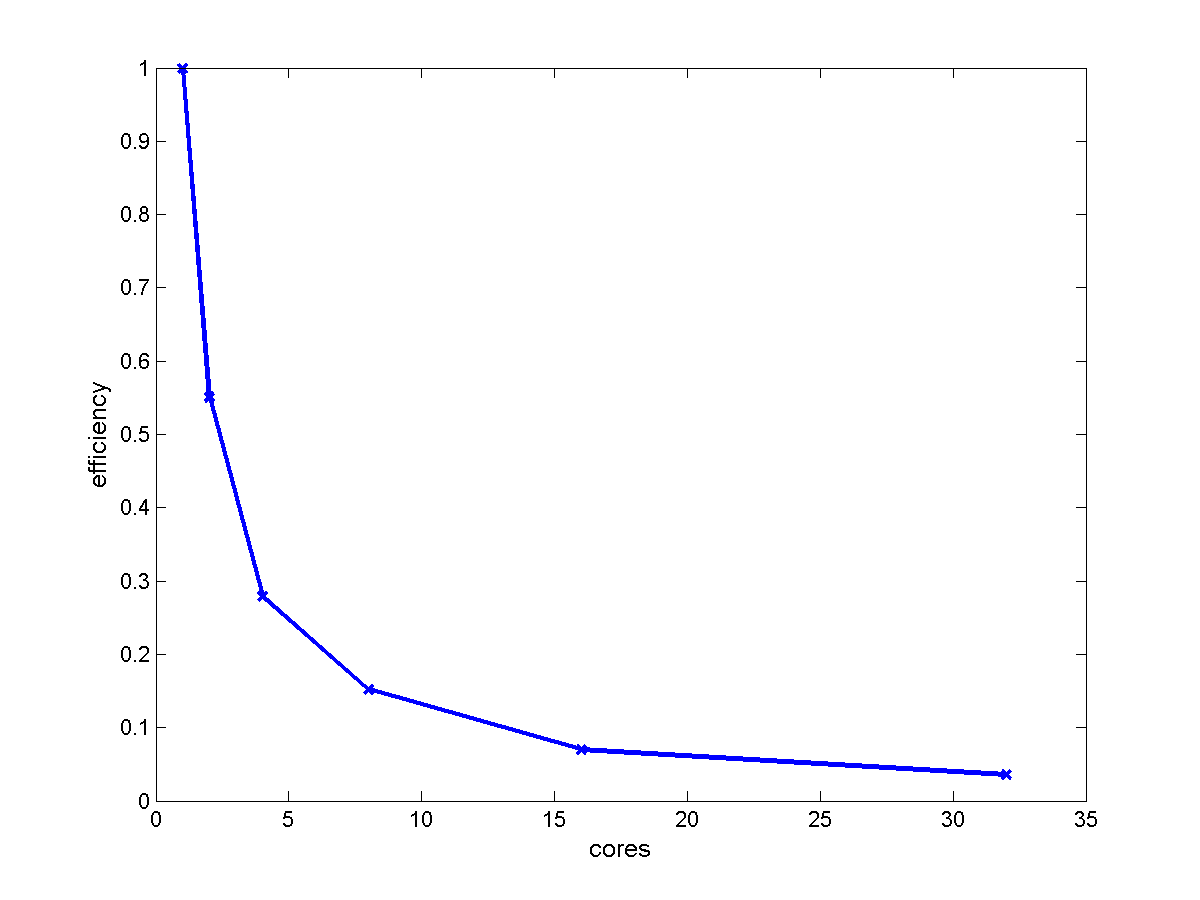
\includegraphics[width=0.3\textwidth]{mcg7_efficiency.png} \\
(a) & (b) & (c) \\
\end{tabular}
\caption{Plots of (a) runtime, (b) speedup, and (c) efficiency for
         MCG-7 with support 0.1.}
\label{fig:mcg7}
\end{figure}
